% Ramin Buzarpur
% student id : 402541206
% final project 

\documentclass[12pt]{article}
\usepackage[utf8]{inputenc}
\usepackage{listings}
\usepackage{xcolor}
\usepackage{hyperref}
\usepackage{graphicx}
\lstdefinelanguage{yaml}{
    keywords={true,false,null,y,n},
    keywordstyle=\color{blue},
    basicstyle=\ttfamily\small,
    sensitive=false,
    comment=[l]{\#},
    commentstyle=\color{gray},
    stringstyle=\color{red},
    morestring=[b]',
    morestring=[b]"
}

\title{Git, GitHub, Vim, and Bash}
\author{}
\date{}

\begin{document}

\maketitle

\section*{Table of Contents}
\begin{enumerate}
    \item \textbf{1. Git and GitHub}
    \begin{enumerate}
        \item 1.1 Repository Initialization and Commits
        \item 1.2 GitHub Actions for LaTeX Compilation
    \end{enumerate}
    \item \textbf{2. Exploration Tasks}
    \begin{enumerate}
        \item 2.1 Vim Advanced Features
        \item 2.2 Memory Profiling
        \begin{enumerate}
            \item 2.2.1 Memory Leak
            \item 2.2.2 Memory Profilers (Valgrind)
        \end{enumerate}
        \item 2.3 GNU/Linux Bash Scripting
        \begin{enumerate}
            \item 2.3.1 fzf
            \item 2.3.2 Using fzf to Find Your Favorite PDF
            \item 2.3.3 Opening the File Using Zathura
        \end{enumerate}
    \end{enumerate}
    \item \textbf{3. Git and FOSS}
    \begin{enumerate}
        \item 3.1 README.md
        \item 3.2 Issues
        \item 3.3 FOSS Contribution
    \end{enumerate}
    \item \textbf{Conclusion}
\end{enumerate}

\newpage

\section*{1.1 Setting up a Repository and Committing Changes}
Setting up a Git repository involves several steps:
\begin{enumerate}
    \item \textbf{Installing Git:}
    Install Git on your system if it’s not already installed:
    \begin{itemize}
        \item Linux:
        \begin{lstlisting}[language=bash]
sudo apt update
sudo apt install git
        \end{lstlisting}
        \item Windows/macOS: Download Git from \url{https://git-scm.com}.
    \end{itemize}
    \item \textbf{Initializing a Repository:}
    Navigate to your project directory and initialize a repository:
    \begin{lstlisting}[language=bash]
cd /path/to/project
git init
    \end{lstlisting}
    \item \textbf{Configuring Git:}
    Set your username and email:
    \begin{lstlisting}[language=bash]
git config --global user.name "Your Name"
git config --global user.email "your-email@example.com"
    \end{lstlisting}
    \item \textbf{Staging and Committing Changes:}
    Add and commit files:
    \begin{lstlisting}[language=bash]
git add .
git commit -m "Initial commit"
    \end{lstlisting}
    \item \textbf{Connecting to GitHub:}
    Add a remote and push changes:
    \begin{lstlisting}[language=bash]
git remote add origin https://github.com/username/repository.git
git push -u origin master
    \end{lstlisting}
\end{enumerate}

\section*{1.2 GitHub Actions for LaTeX Compilation}
GitHub Actions automates LaTeX document compilation. Steps:
\begin{enumerate}
    \item Create a workflow file in \texttt{.github/workflows/latex.yml}.
    \item Use the following configuration:
    \begin{lstlisting}[language=yaml]
name: Compile LaTeX

on:
  push:
    branches:
      - main

jobs:
  build:
    runs-on: ubuntu-latest

    steps:
      - uses: actions/checkout@v3
      - uses: dante-ev/latex-action@v2
        with:
          root_file: main.tex
          latexmk_shell_escape: true
    \end{lstlisting}
\end{enumerate}

\section*{2.1 Advanced Features of Vim}
\begin{enumerate}
    \item \textbf{Macros:} Record and replay commands with \texttt{q}.
    \item \textbf{Multiple Cursors:} Use the \texttt{vim-multiple-cursors} plugin.
    \item \textbf{Registers:} Save and retrieve text blocks.
\end{enumerate}

\section*{2.2 Memory Profiling}
\subsection*{2.2.1 Memory Leaks}
Memory leaks occur when dynamically allocated memory is not freed, leading to inefficiencies.

\subsection*{2.2.2 Valgrind}
Detect memory leaks with:
\begin{lstlisting}[language=bash]
gcc -g -o program program.c
valgrind --leak-check=full ./program
\end{lstlisting}

\section*{2.3 Bash Scripting}

\subsection*{2.3.1 fzf}
\textbf{Fuzzy Searching:} Fuzzy searching is a technique used to find approximate matches rather than exact ones. This is particularly useful when you don't remember the exact name of a file, command, or data.

\subsubsection*{What does \texttt{ls | fzf} do?}
The command \texttt{ls | fzf}:
\begin{itemize}
    \item Lists all files and directories in the current directory using \texttt{ls}.
    \item Pipes the output to \texttt{fzf}, which allows the user to interactively search and select an item.
\end{itemize}

\subsection*{2.3.2 Using fzf to Find Your Favorite PDF}

\subsubsection*{1. Listing all PDF files}
To list all PDF files in the current directory and its subdirectories, use the following command:
\begin{lstlisting}[language=bash]
fd --extension pdf
\end{lstlisting}

\subsubsection*{2. Selecting a PDF using fzf}
To interactively select a PDF file from the list generated above, pipe the output to \texttt{fzf}:
\begin{lstlisting}[language=bash]
fd --extension pdf | fzf
\end{lstlisting}

\subsection*{2.3.3 Opening the File Using Zathura}
To open the selected PDF file using Zathura, combine the above commands as follows:
\begin{lstlisting}[language=bash]
zathura $(fd --extension pdf | fzf)
\end{lstlisting}

\subsubsection*{Explanation of \texttt{\$(command)} Syntax}
The syntax \texttt{\$(command)}:
\begin{itemize}
    \item Runs the command inside the parentheses.
    \item Substitutes the output of the command as an argument for the preceding command.
\end{itemize}
In this case, the command finds and selects a PDF file, and its path is passed to \texttt{zathura} to open it.

\section*{3. Git and FOSS}

\subsection*{3.1 README.md}
A README file is essential for any project. It provides an overview of the project, instructions for use, and other relevant information.

\subsection*{3.2 Issues}
GitHub Issues are a great way to track bugs, feature requests, and other tasks related to a project.

\subsection*{3.3 FOSS Contribution}
Contributing to Free and Open Source Software (FOSS) projects is a valuable way to improve your skills and give back to the community.

\section*{Perspective on FOSS Contributions}
No, I don’t see myself contributing to FOSS (Free and Open Source Software) projects in the future. While I understand the importance of open-source software and the impact it has on the tech industry, I simply don’t have any interest in programming or software development. My passion lies entirely in the field of network security, and I prefer to focus my time and energy on that area.

\section*{Conclusion}
Using \texttt{fzf}, \texttt{fd}, and \texttt{zathura}, we can efficiently search for and open PDF files in seconds. This workflow demonstrates the power of combining CLI tools to simplify complex tasks.

\begin{figure}[h]
    \centering
    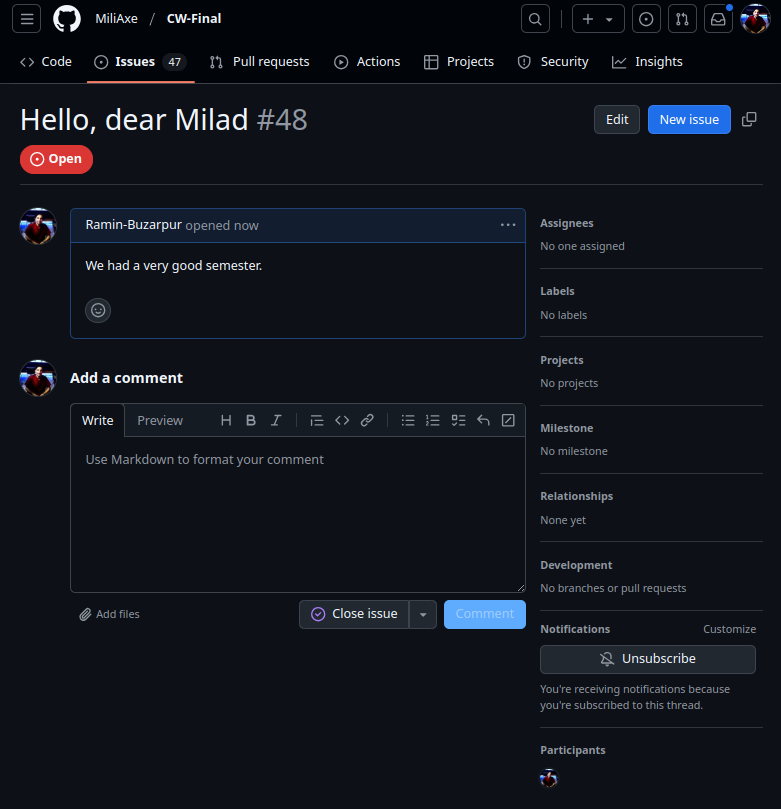
\includegraphics[width=0.8\textwidth]{Screenshot from 2025-01-25 19-40-14.png}
\end{figure}

\end{document}
\end{document}